% sections/05-layered-architecture.tex
% OWNER: Member D
% Do NOT edit this file if you are not Member D.
% Statements marked "our interpretation" are the authors' analysis, not claims made by Uber.

\section{Layered Architecture in Michelangelo}
\label{sec:layered-architecture}

This section analyses Michelangelo's backbone style, the \textbf{layered
architecture}: its definition (\Cref{sec:layered-style}), how Michelangelo maps
onto it (\Cref{sec:layered-mapping}), how the layers communicate
(\Cref{sec:layered-communication}), which other styles live inside the layers
(\Cref{sec:layered-other-styles}) and how well the style serves the platform
(\Cref{sec:layered-evaluation}).

% ------------------------------------------------------------
\subsection{The Layered Architecture Style}
\label{sec:layered-style}

A layered architecture splits a system into horizontal layers. Each layer offers
services to the layer above and uses services of the layer
below~\cite{buschmann1996}. The core rule is a one-way \emph{allowed-to-use}
relation: a layer may use the layers beneath it, never those above
it~\cite{bass2021}. Richards and Ford describe layering as one of the most common
styles. They call it \emph{technically partitioned}, meaning the system is divided
by technical role rather than by business domain~\cite{richards2020}.

Two design rules shape a layered system~\cite{richards2020}:
\begin{itemize}
  \item \textbf{Closed vs.\ open layers.} A \emph{closed} layer cannot be
        skipped; an \emph{open} one can. Closed layers create \emph{isolation}:
        changes inside a layer do not ripple outward.
  \item \textbf{Separation of concerns.} Each layer has one job and can be
        built, tested and replaced on its own.
\end{itemize}

\textbf{Benefits:} easy to understand and split among teams; a layer can be
replaced behind a stable interface; lower layers are
reusable~\cite{richards2020,bass2021}.

\textbf{Liabilities:} each crossed layer adds latency; cross-cutting changes touch
every layer; requests may pass through layers that add no logic (the
\emph{architecture sinkhole} anti-pattern); strict layering feels
rigid~\cite{richards2020,bass2021}.

% ------------------------------------------------------------
\subsection{Mapping Michelangelo onto Layers}
\label{sec:layered-mapping}

\subsubsection{How the layers emerged}
\begin{itemize}
  \item \textbf{2017 (1.0).} ML components (feature store, training, model
        repository, prediction service) ran on ``a mix of open source systems
        and components built in-house'' such as HDFS, Spark, Samza and
        Cassandra, managed by an API tier, web UI and workflow
        system~\cite{uber2017}.
  \item \textbf{2018.} Uber began ``factoring out Michelangelo's infrastructure
        into an explicit infrastructure layer'' so other teams could ``build
        more specialized platforms'' on top of it~\cite{uber2018}.
  \item \textbf{2024 (2.0).} The architecture is described as \textbf{three
        planes} (control, offline data and online data) built on a bottom layer
        of \textbf{plug-and-play components}~\cite{uber2024}.
\end{itemize}

\subsubsection{Our five-layer view}
To Uber's three planes and plug-and-play components~\cite{uber2024} \textbf{we
add two layers of our own}, built from components Uber names: an
\emph{experience layer} (MA Studio, Canvas) on top and an \emph{infrastructure
layer} (clusters, GPUs, storage) at the bottom (\Cref{fig:layered-view}).

\begin{figure}[ht]
  \centering
  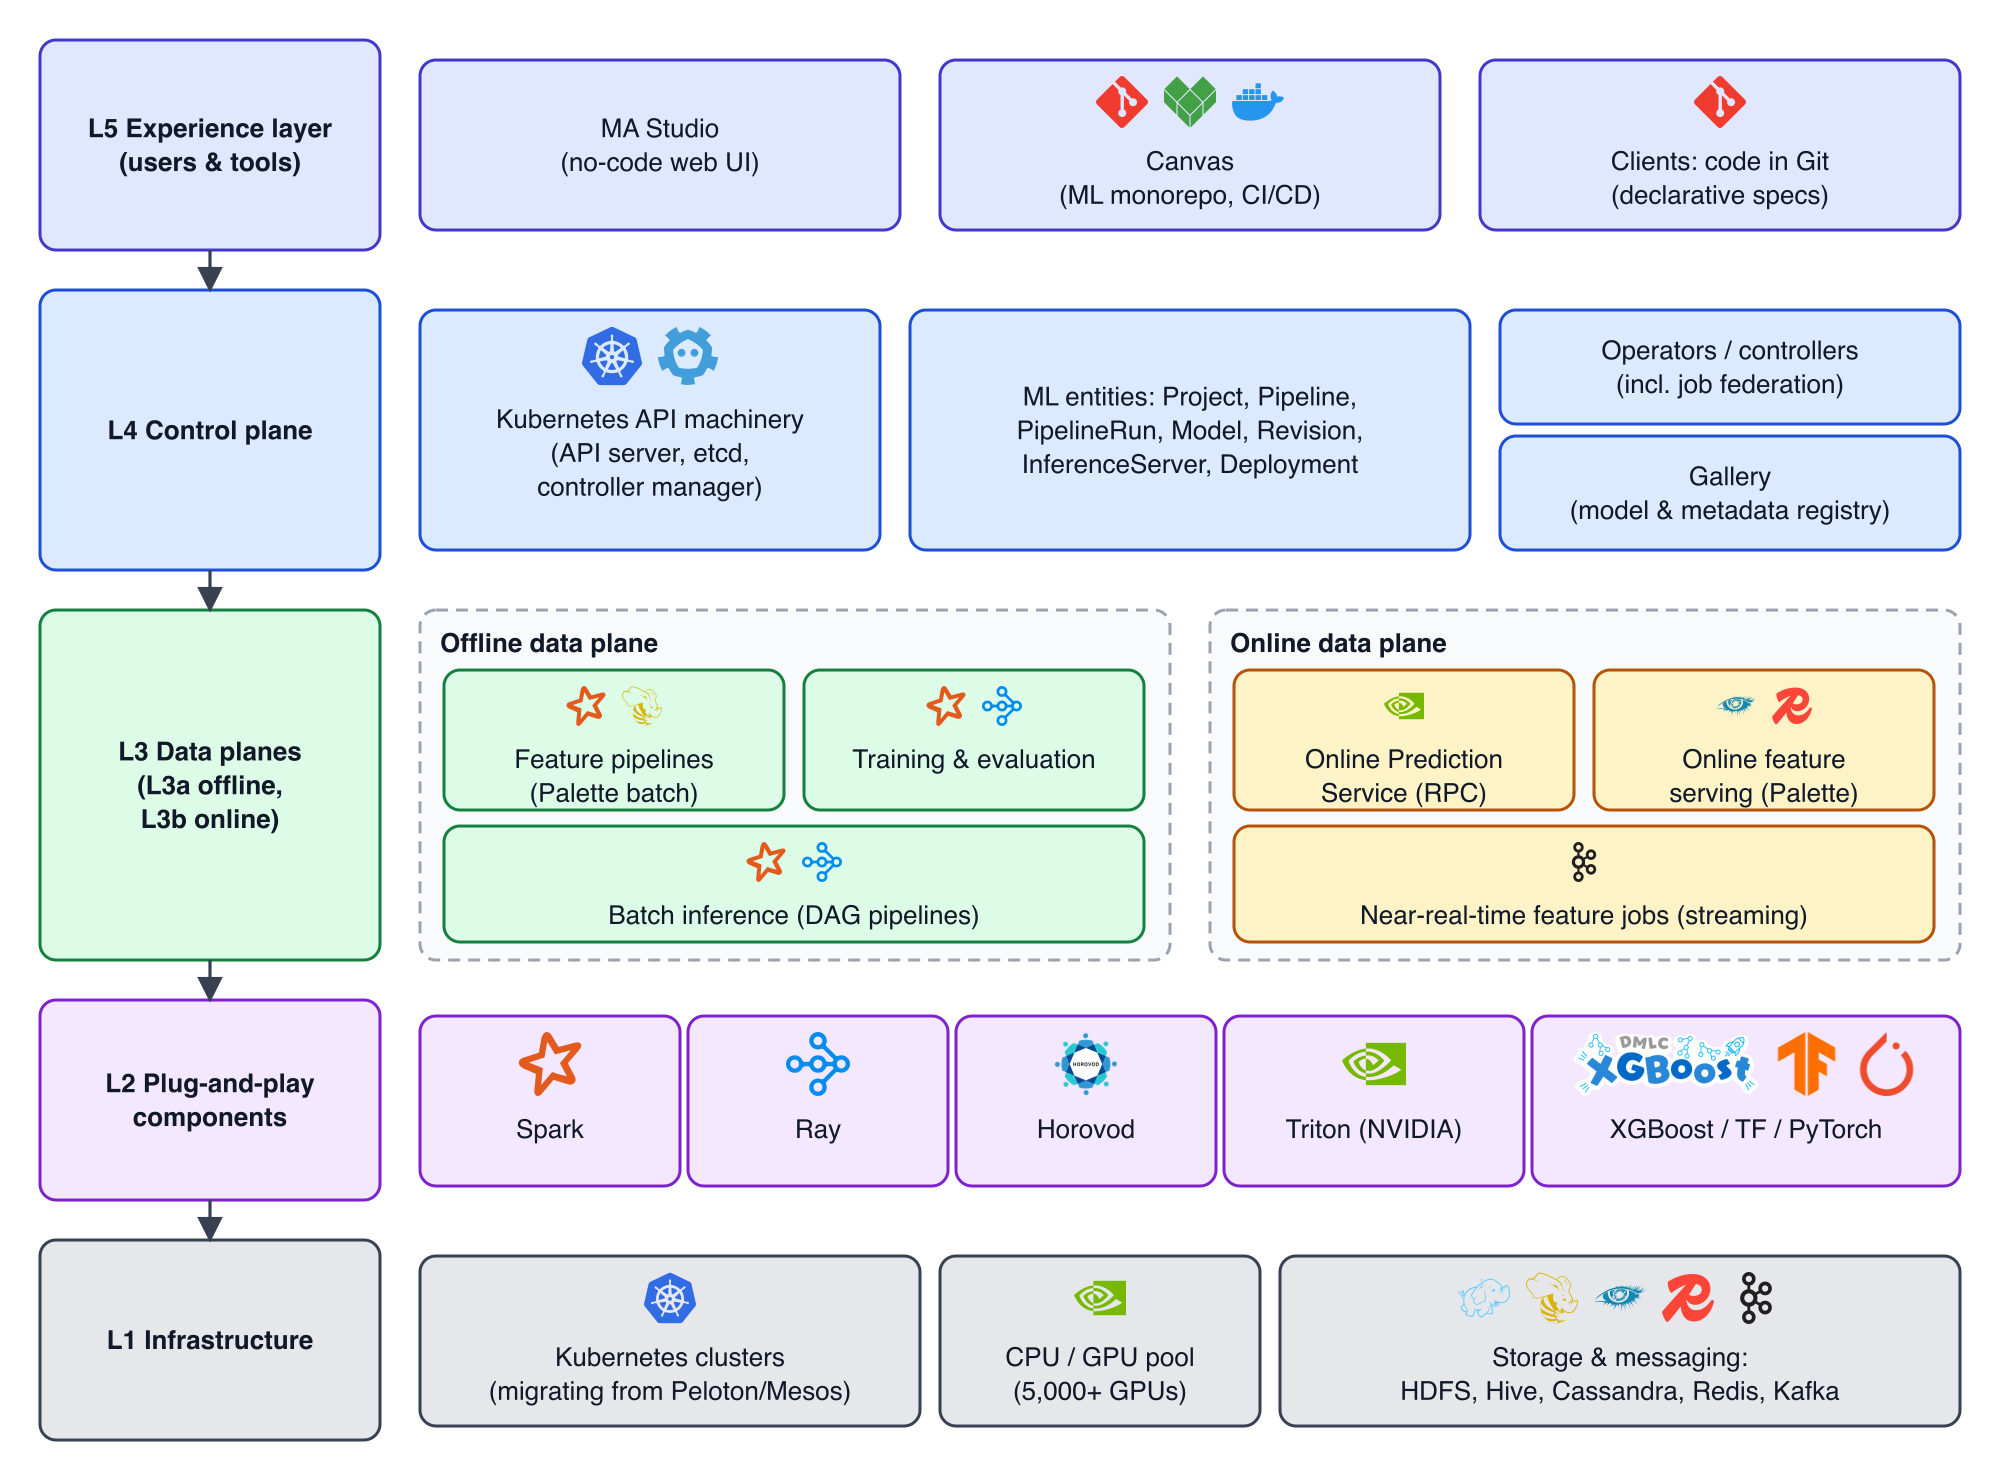
\includegraphics[width=\linewidth]{memberD-fig5-1-layered-view}
  \caption[Layered view of Michelangelo 2.0]{Layered view of Michelangelo 2.0.
    Each arrow means ``uses'' (top-down only). The offline and online data
    planes are peers inside layer L3.}
  \label{fig:layered-view}
\end{figure}

\begin{table}[ht]
  \centering
  \small
  \caption{Responsibilities, components and technologies of each layer.}
  \label{tab:layers}
  \begin{tabularx}{\linewidth}{@{}L{2.3cm}*{3}{>{\raggedright\arraybackslash}X}@{}}
    \toprule
    \textbf{Layer} & \textbf{Responsibility} & \textbf{Main components} & \textbf{Technologies} \\
    \midrule
    L5 Experience & Define and inspect ML work
      & MA Studio (no-code UI), Canvas (ML monorepo, CI/CD)
      & Web UI, Git, Bazel, Docker~\cite{uber2024} \\
    L4 Control plane & User-facing APIs; lifecycle of all ML entities
      & API server, controllers, job federation, Gallery
      & Kubernetes API server, etcd, controller manager~\cite{uber2024} \\
    L3a Offline data plane & Features, training, evaluation, batch inference
      & Palette batch pipelines, training pipelines, batch scoring
      & Spark, Ray~\cite{uber2024}; Hive/HDFS~\cite{uber2017} \\
    L3b Online data plane & Real-time inference and feature serving
      & Online prediction service, online feature serving, streaming feature jobs
      & Triton~\cite{uber2024}; Cassandra/Redis~\cite{uber2024palette};
        Kafka, Samza~\cite{uber2017} \\
    L2 Plug-and-play & Swappable engines
      & Compute and serving engines, ML frameworks
      & Spark, Ray, Horovod, Triton, XGBoost, TensorFlow,
        PyTorch~\cite{uber2024} \\
    L1 Infrastructure & Compute, storage, messaging
      & Clusters, CPU/GPU pool, storage
      & Kubernetes (from Peloton/Mesos), 5,000+ GPUs~\cite{uber2024};
        HDFS, Cassandra, Kafka~\cite{uber2017} \\
    \bottomrule
  \end{tabularx}
\end{table}

\paragraph{Control plane (L4).}
\begin{itemize}
  \item It ``defines user-facing APIs and manages the lifecycle of all entities
        in the system''~\cite{uber2024}.
  \item It follows the Kubernetes Operator pattern and Kubernetes API
        conventions, using the API server, etcd and controller
        manager~\cite{uber2024}.
  \item Its standard ML entities are Project, Pipeline, PipelineRun, Model,
        Revision, InferenceServer and Deployment~\cite{uber2024}. \emph{Our
        interpretation:} given the Kubernetes conventions and the named ``job
        CRD controller''~\cite{uber2024}, they are likely Kubernetes custom
        resources, as Palette's Feature and FeatureStore
        are~\cite{uber2024palette}.
  \item The API is \emph{declarative}: users state the desired result, and
        controllers make reality match it. Changes can come from the UI or from
        code in Git~\cite{uber2024}.
  \item The \emph{job federation} controller spreads Spark and Ray jobs across
        clusters, hiding ``the region, and zone and cluster
        details''~\cite{uber2024}.
  \item Gallery is the model and metadata registry~\cite{uber2024}. It continues
        1.0's versioned model repository, which stored each model's
        configuration, metrics and parameters~\cite{uber2017}.
\end{itemize}

\paragraph{Offline data plane (L3a).}
\begin{itemize}
  \item It ``does the heavy lifting on big data processing'': features,
        training, evaluation and batch inference~\cite{uber2024}.
  \item Work runs as pipelines, which are DAGs of steps executed on Spark or
        Ray. Checkpoints let a pipeline resume without repeating finished
        steps~\cite{uber2024}.
  \item Palette supports batch feature pipelines~\cite{uber2024}, and offline
        features are kept as daily Hive snapshots~\cite{uber2024palette}.
\end{itemize}

\paragraph{Online data plane (L3b).}
\begin{itemize}
  \item It ``handles real-time model inference and feature serving'' for Uber's
        other microservices, through RPC services and streaming
        jobs~\cite{uber2024}.
  \item The Online Prediction Service (OPS) now uses Triton, which Uber
        describes as optimised for low-latency GPU serving~\cite{uber2024}.
  \item Online features live in Cassandra or Redis~\cite{uber2024palette}.
  \item In 2017, P95 latency was under 5\,ms for models without
        Cassandra-backed features and under 10\,ms with
        them~\cite{uber2017}. By 2024 the platform served 10 million
        predictions per second at peak~\cite{uber2024}.
\end{itemize}

% ------------------------------------------------------------
\subsection{Dependencies and Communication Between Layers}
\label{sec:layered-communication}

Dependencies point strictly \textbf{top-down}: upper layers command lower ones,
and lower layers never call upward. Information returns upward only in two ways:
\begin{itemize}
  \item as \textbf{status} written back to control-plane resources (Kubernetes
        convention~\cite{uber2024});
  \item as \textbf{data} left in shared storage.
\end{itemize}
\Cref{fig:layered-communication} traces the main interactions.

\begin{figure}[ht]
  \centering
  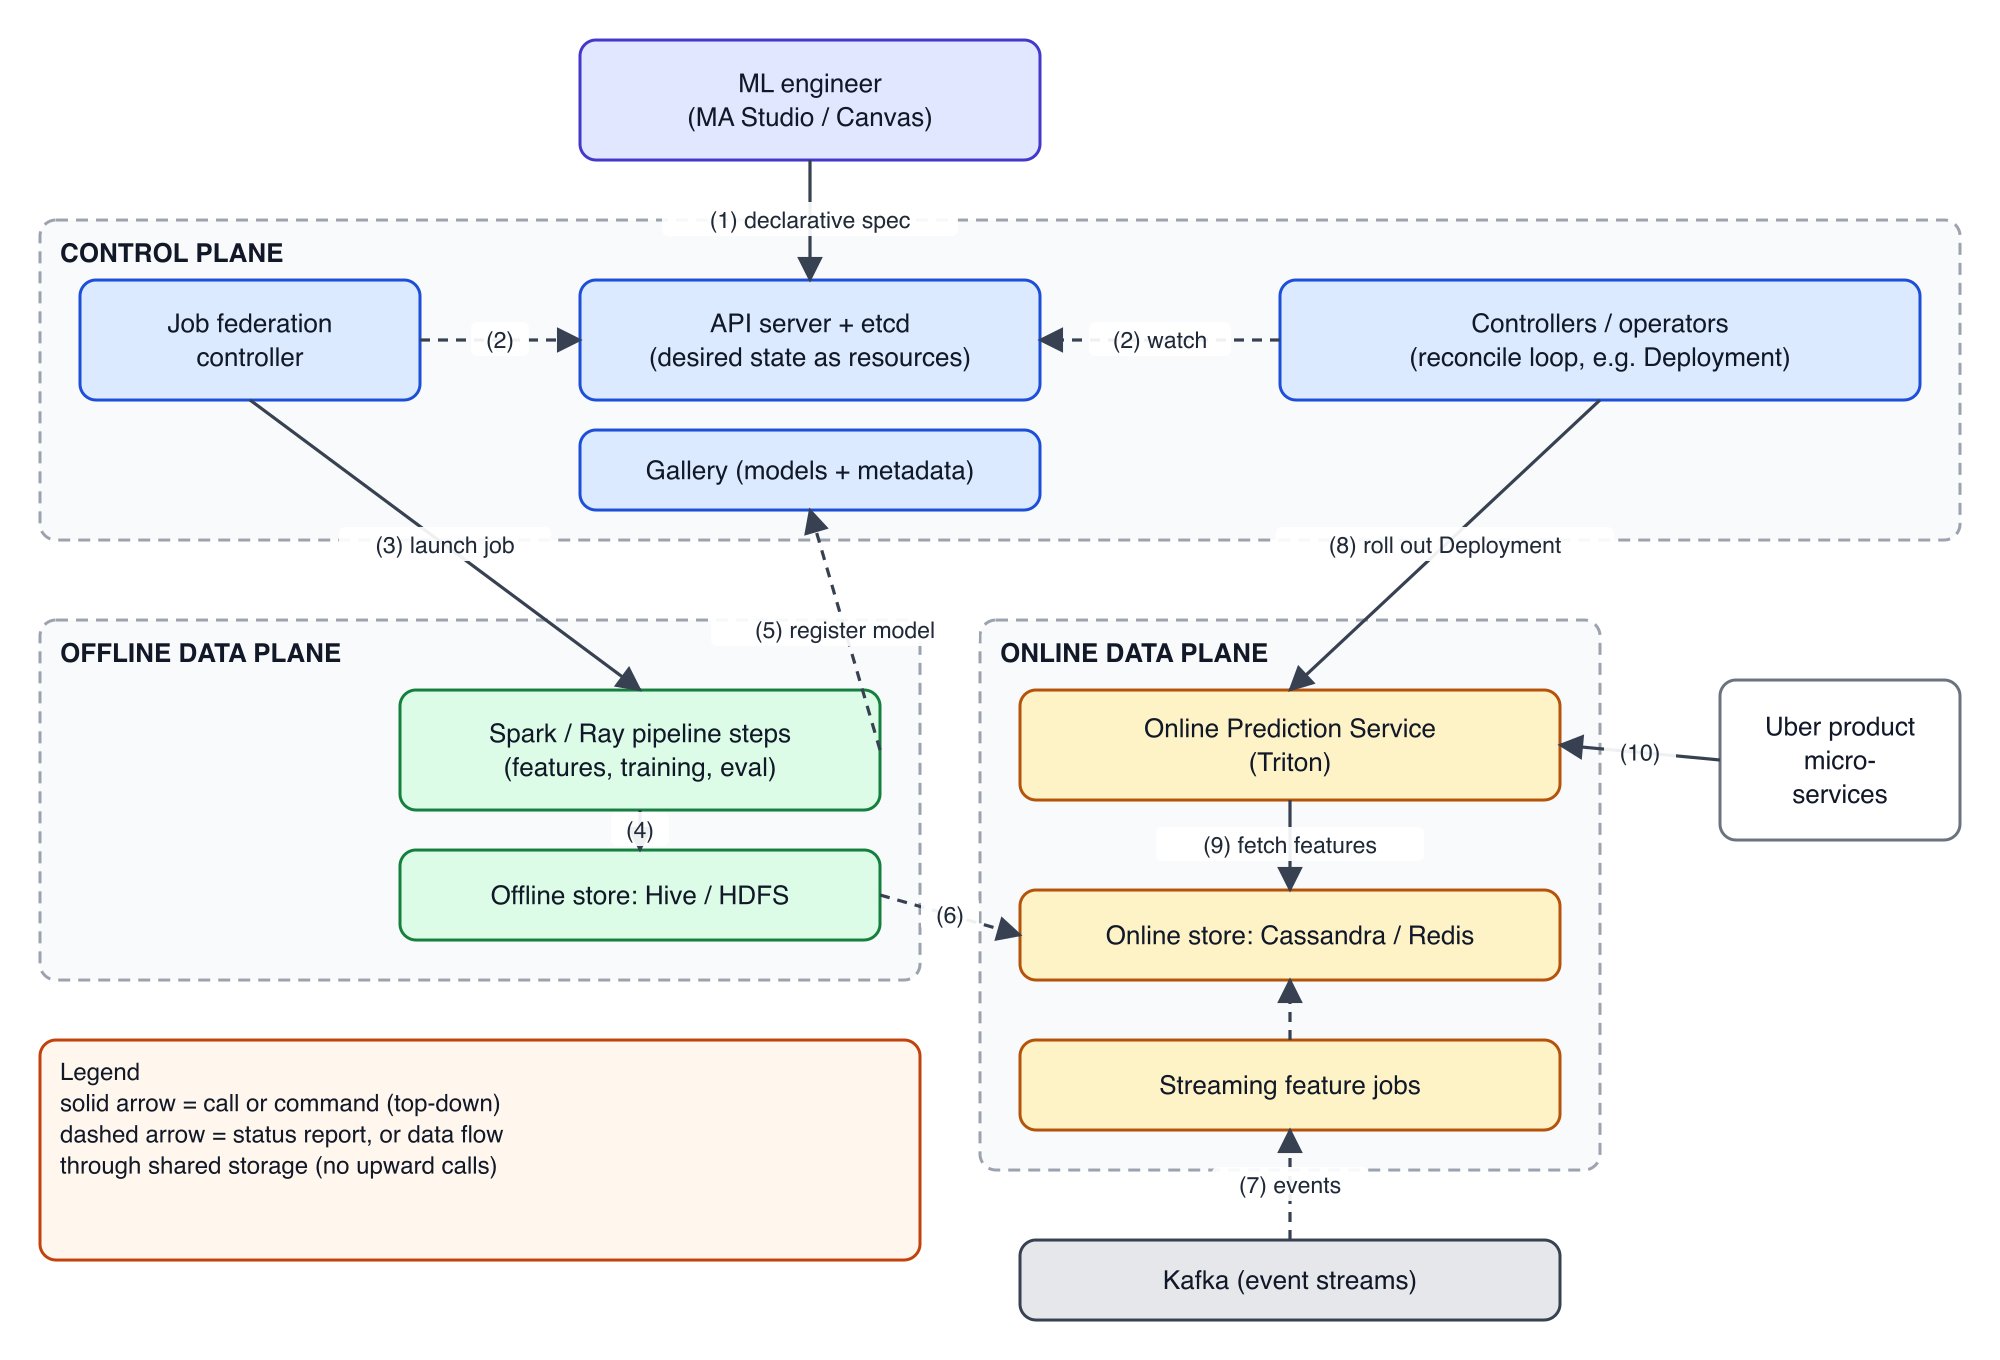
\includegraphics[width=\linewidth]{memberD-fig5-2-communication}
  \caption[Dependencies and communication between the layers]{Dependencies and
    communication between the layers. Solid arrows are calls or commands;
    dashed arrows are status reports or data handed over through storage.}
  \label{fig:layered-communication}
\end{figure}

\begin{enumerate}
  \item An ML engineer submits a desired state (e.g.\ a Pipeline or Deployment)
        from MA Studio or Canvas~\cite{uber2024}.
  \item Controllers watch the API server, act to close the gap between desired
        and actual state, and report status~\cite{uber2024}.
  \item The job federation controller launches Spark or Ray jobs on any
        suitable cluster~\cite{uber2024}.
  \item Pipeline steps read the data lake and write features to the offline
        store~\cite{uber2017}.
  \item Training stores the model, its configuration and metrics as a new
        version in the model repository, which is Gallery in
        2.0~\cite{uber2017,uber2024}. This is a write into a shared store
        (Cassandra in 2017), not a call to the control plane's logic.
  \item \emph{Batch path:} historical features are loaded from HDFS into
        Cassandra~\cite{uber2017}.
  \item \emph{Speed path:} streaming jobs aggregate Kafka events into
        Cassandra~\cite{uber2017}.
  \item A controller rolls the model out to OPS, with ``safe and incremental
        zonal rollout'' and automatic rollback~\cite{uber2024}. Models are
        referenced by ID or tag, enabling side-by-side versions and A/B
        tests~\cite{uber2017}.
  \item At prediction time, the model's features are read from
        Cassandra~\cite{uber2017}.
  \item Uber's product microservices call the prediction service over
        RPC~\cite{uber2017,uber2024}.
\end{enumerate}

Two observations follow:
\begin{itemize}
  \item \textbf{The two data planes never call each other.} They share data
        through storage (steps 6--7) and are coordinated from above (steps 3
        and 8), so the online plane is independent of batch jobs.
  \item \textbf{Closed and open layers.} The control plane is \emph{closed}:
        every change goes through its declarative API. The plug-and-play layer
        is partly \emph{open}: the managed solution supports a curated subset,
        but advanced users can ``bring your own components''~\cite{uber2024}.
\end{itemize}

% ------------------------------------------------------------
\subsection{Other Architecture Styles Inside the Layers}
\label{sec:layered-other-styles}

Layering is Michelangelo's backbone, but each layer uses the style that fits its
job (\Cref{fig:layered-styles}).

\begin{figure}[ht]
  \centering
  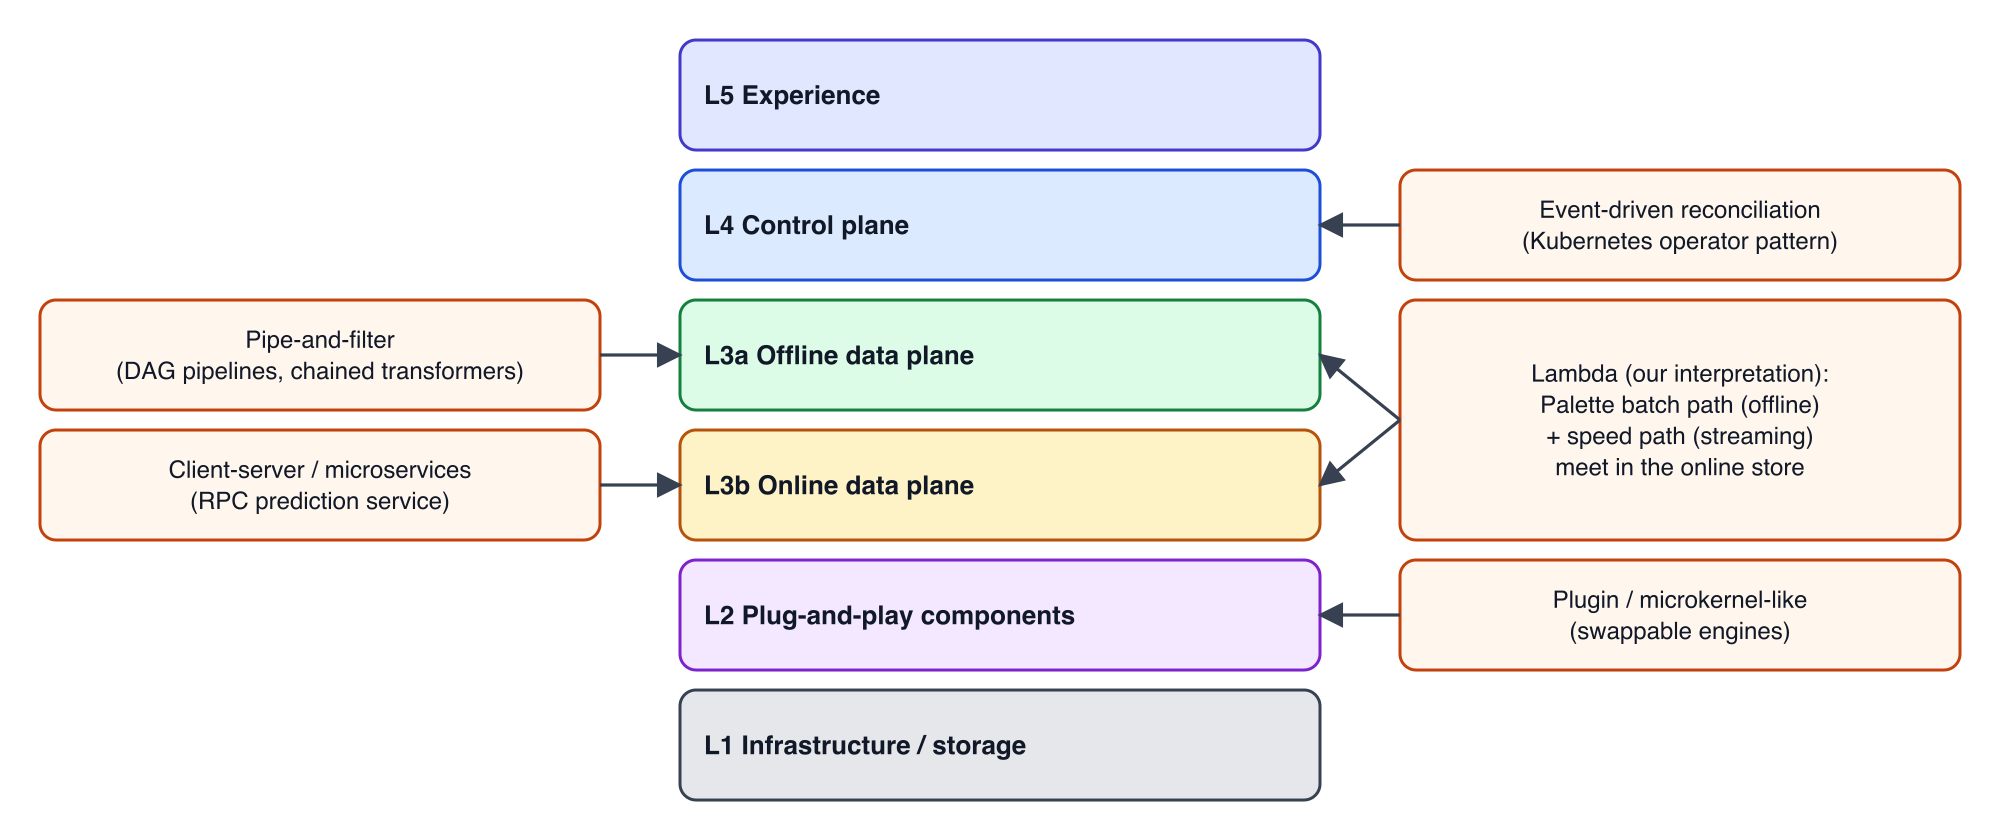
\includegraphics[width=\linewidth]{memberD-fig5-3-styles-in-layers}
  \caption[Other architecture styles placed in the layers]{Other architecture
    styles placed in the layers.}
  \label{fig:layered-styles}
\end{figure}

\begin{itemize}
  \item \textbf{Pipe-and-filter: offline data plane.} Pipelines are DAGs of
        steps, each consuming earlier outputs~\cite{uber2024}. Feature
        transformers are chained before the model, and Triton joined OPS as
        ``a new Spark transformer''~\cite{uber2024}.
  \item \textbf{Lambda: Palette, spanning both data planes} (\emph{our
        interpretation}). Batch and speed paths meet in a single serving
        store, Cassandra~\cite{uber2017}. This matches Lambda's batch, speed
        and serving layers, although Uber never uses the term.
  \item \textbf{Event-driven reconciliation: control plane.} Following the
        Kubernetes Operator pattern, controllers react to resource
        changes~\cite{uber2024}.
  \item \textbf{Plugin (microkernel-like): plug-and-play layer.}
        Plug-and-play is one of Uber's six design principles. Stable
        entities hide interchangeable engines~\cite{uber2024}.
  \item \textbf{Client-server / microservices: online data plane.} The
        prediction service answers RPC calls from other Uber
        services~\cite{uber2017}.
\end{itemize}

Layering decides \emph{what may depend on what}; each layer picks the style that
serves its own goal.

% ------------------------------------------------------------
\subsection{Evaluation: How Well Does Layering Serve Michelangelo?}
\label{sec:layered-evaluation}

\subsubsection{Benefits}

\paragraph{Benefit 1. Lower layers change without disturbing upper layers.}
Uber is migrating its clusters from Peloton/Mesos to Kubernetes and extending to
cloud GPUs on OCI and GCP~\cite{uber2024}. The job federation layer hides
cluster details for ``job portability''~\cite{uber2024}, so engineers keep
submitting the same pipelines while the infrastructure underneath changes. This
is the isolation the style promises~\cite{richards2020}.

\paragraph{Benefit 2. Engines are swapped inside a layer.}
\begin{itemize}
  \item Neuropod ``lacks continuous community support and is being
        deprecated'', so Triton replaced it in OPS~\cite{uber2024}.
  \item Uber ``replaced Spark-based XGBoost and DL trainers with Ray-based
        trainers \ldots{} for better scalability and reliability''. The earlier
        Horovod-on-Spark setup had ``introduced many operational
        complexities''~\cite{uber2024}. Horovod itself remains the distributed
        training framework~\cite{uber2024}.
  \item \emph{Our interpretation:} teams describe \emph{what} to train and
        deploy (Pipeline, Model, Deployment), not \emph{which engine} runs it,
        so these swaps stayed inside the lower layers.
\end{itemize}

\paragraph{Benefit 3. Reuse at scale.}
The 2018 infrastructure layer let teams build specialised platforms on
it~\cite{uber2018}. By 2024 one platform carried about 400 projects, 20,000+
training jobs per month and 5,000+ production models~\cite{uber2024}.

\subsubsection{Limitations}

\paragraph{Limitation 1. A fault in a shared lower layer spreads upward.}
\begin{itemize}
  \item \emph{What happened:} in 2021, a bad Palette metadata change stopped
        online serving from loading metadata at boot, breaking major Tier-1 use
        cases~\cite{uber2024palette}.
  \item \emph{Why:} schema validation ran client-side, so users on outdated
        code merged incorrect metadata. With no incremental update system,
        changing one feature group triggered updates to hundreds of
        them~\cite{uber2024palette}.
  \item \emph{Fix:} server-side validation, Feature and FeatureStore CRDs, a
        Kubernetes-based controller and delta propagation. End-to-end updates
        dropped from ``over an hour'' to about 15
        minutes~\cite{uber2024palette}.
  \item \emph{Our interpretation:} this is the classic layering risk. A layer
        that many others depend on needs stronger safeguards than any single
        caller.
\end{itemize}

\paragraph{Limitation 2. Extra hops cost latency} (\emph{our interpretation} of
Uber's data). Models that read features from the Cassandra storage layer had a
P95 target of under 10\,ms, against under 5\,ms for models that did
not~\cite{uber2017}. Every hop into a lower layer on the request path consumes
latency budget.

\paragraph{Limitation 3. Rigidity and cross-layer change.}
\begin{itemize}
  \item Michelangelo 1.0's config- and UI-driven path slowed iteration. Uber's
        lesson was ``let developers use the tools that they want'', which led
        it to add PyML~\cite{uber2018}.
  \item The Spark-based feature transformation DSL could not run on GPUs, which
        limited low-latency deep-learning serving~\cite{uber2024}. A concern
        shared by several layers needs coordinated change across all of them.
  \item Uber's answer was to open layers selectively (Canvas, ``bring your own
        components'')~\cite{uber2024}.
\end{itemize}

\subsubsection{Overall assessment}
Layering isolates fast-changing infrastructure and engines from hundreds of
product teams and lets one platform be shared at scale. Its costs are the
classic ones: fragile shared layers, latency per hop and rigidity. Uber kept the
layers and managed these costs with stronger validation in shared layers, a
separate online plane and deliberately opened layers. \emph{Our
interpretation:} the move from the loosely layered 1.0 to the explicit
three-plane 2.0 suggests that a large MLOps platform benefits from \emph{more}
layering discipline over time, not less.
